\documentclass{article}
\usepackage{ctex}
\usepackage{fontspec}
\usepackage{listings}
\usepackage{xcolor}
\usepackage{geometry}
\usepackage{graphicx}
\usepackage{float}
\usepackage{amsmath}
\usepackage{minted}
\geometry{a4paper,scale=0.8}
\definecolor{codebg}{rgb}{0.95,0.95,0.95}
\begin{document}
\title*{\Huge \centering \vfill \textbf{实验1 \ KNN(K近邻算法)}}
\section*{\LARGE 一、实验目的}
K近邻(KNN)算法是一种常用的监督学习算法,它通过计算待分类样本与训练集中各个样本之间的距离,
选择距离最近的K个样本作为待分类样本的“邻居”,然后通过这些邻居的分类情况来确定待分类样本的类别。
KNN算法简单易懂,效果较好,并且由于KNN没有显式的学习过程,不需要花费大量的时间用于样本训练,
在实际应用中也有广泛的应用。


本实验旨在了解K近邻(KNN)算法的基本原理和应用,熟悉数据预处理和模型评估的方法,以及掌握python等科学
编程语言在机器学习中的应用

\section*{\LARGE 二、实验原理}
K近邻(KNN)算法是一种基于实例的学习方法,它通过计算待分类样本与训练集中各个样本之间的距离,选择距离最近的K个样本作为待分类样本的“邻居”,然后通过这些邻居的分类情况来确定待分类样本的类别。
具体而言,假设我们有一个训练集$D=\{(x_1,y_1),(x_2,y_2),\cdots,(x_n,y_n)\}$,其中$x_i=(x_{i1},x_{i2},\cdots,x_{im})$表示第$i$个样本的$m$个特征值,$y_i$为该样本的类别。对于一个待分
类的样本$x$,我们需要计算它与训练集中各个样本的距离,通常使用欧氏距离$(Euclidean\ Distance)$
$$d(x_i,x_j)=\sqrt{\sum_{k=1}^m(x_{ik}-x_{jk})^2}$$
或曼哈顿距离$(Manhattan\ Distance)$
$$d(x_i,x_j)={\sum_{k=1}^m|x_{ik}-x_{jk}|}$$
这里我们把上述两种常见的距离计算公式统一归为$Minkowski\ Distance$的$p=2$和$p=1$的特殊情况
$$d(x_i,x_j)={(\sum_{k=1}^m|x_{ik}-x_{jk}|^p)^{\frac{1}{p}}}$$


计算出距离后,我们选择距离最近的K个样本作为待分类样本的邻居,然后通过这些邻居的分类情况来确定待分类样本的类别。通常采用多数表决的方法,即选择K个邻居中出现次数最多的类别作为待分类样本的类别,例如:
$$y=\arg\max_{c_j}\sum_{i=1}^KI(y_i=c_j)$$
其中$I$表示指示函数,当$y_i=c_j$时,$I(y_i=c_j)=1$,否则$I(y_i=c_j)=0$。
需要注意的是,KNN算法需要选择合适的K值,通常可以通过交叉验证等方法来确定;如果数据规模较小,也可以选定一个值的附近范围逐一尝试。当K值较小时,模型的复杂度较高,容易受到噪声等因素的影响;当K值较大时,
模型的复杂度较低,但容易出现欠拟合的情况。因此,选择合适的K值非常重要。另外,KNN算法也需要对数据进行预处理,例如归一化、标准化等操作,以确保不同特征之间的尺度一致,从而避免某些特征对模型的影响过大。
综上所述,KNN算法是一种简单而有效的分类算法,它的原理简单易懂,应用广泛。在实际应用中,我们需要根据具体的问题选择合适的距离度量方法等以获得更好的分类效果。

\section*{\LARGE 三、实验步骤}\noindent
1、利用python的numpy模块完成KNN算法。\\
2、使用随机分布函数生成训练数据和测试数据。\\
3、完成结果的可视化,报告准确率。\\

\section*{\LARGE 四、实验代码}\noindent
变量定义与声明,这里我们默认生成$1800$个训练样本点,测试样本点为$100$个,根据不同的点所在的区域,指定不同的$tag$。
\begin{minted}[linenos,breaklines,bgcolor=codebg]{python3}
import numpy as np
import matplotlib.pyplot as plt

np.random.seed(25565)
sample=np.random.rand(1800,2)*10
tag=np.zeros(1800)
test=np.random.rand(100,2)*10
test_tag=np.zeros(100)
default_color= ['#1f77b4', '#ff7f0e', '#2ca02c', '#d62728', '#9467bd', '#8c564b', '#e377c2', '#7f7f7f', '#bcbd22', '#17becf']

total_samplenum=0
\end{minted}
\noindent KNN算法的实现
\begin{minted}[linenos,breaklines,bgcolor=codebg]{python3}
def sort_key(item:tuple):
    return item[0]

def knn_predict(point:np.array,n:int)->int:
    dist:list=[]
    for k in range(1,len(sample)):
        if sample[k][0]==-1:
            continue
        eu_dis=(sample[k]-point)@(sample[k]-point)
        man_dis=np.sum(np.abs(sample[k]-point))
        inf_dis=np.max(np.abs(sample[k]-point))
        dist.append((eu_dis,int(tag[k])))
    dist.sort(key=sort_key)
    vote:list=dist[0:n]
    result=np.zeros(10)
    for j in range(0,len(vote)):
        result[vote[j][1]]+=1
    return result.argmax()
\end{minted}
\noindent 训练样本和测试样本的生成与划分,本实验中,每个类的样本点范围是$3\times 3$区域,相邻的类之间间隔距离为$0.5$。
\begin{minted}[linenos,breaklines,bgcolor=codebg]{python3}
for i in range(0,len(sample)):
    if((sample[i][0]>=3 and sample[i][0]<=3.5) or (sample[i][0]>=6.5 and sample[i][0]<=7)
        or (sample[i][1]>=3 and sample[i][1]<=3.5) or (sample[i][1]>=6.5 and sample[i][1]<=7)):
        sample[i]=np.array([-1,-1])
        continue
    if(sample[i][0]>=0 and sample[i][0]<=3 and sample[i][1]>=0 and sample[i][1]<=3):
        tag[i]=1
        plt.scatter(sample[i][0],sample[i][1],marker='3',c=default_color[0])
    elif(sample[i][0]>=3.5 and sample[i][0]<=6.5 and sample[i][1]>=0 and sample[i][1]<=3):
        tag[i]=2
        plt.scatter(sample[i][0],sample[i][1],marker='3',c=default_color[1])
    elif(sample[i][0]>=7 and sample[i][0]<=10 and sample[i][1]>=0 and sample[i][1]<=3):
        tag[i]=3
        plt.scatter(sample[i][0],sample[i][1],marker='3',c=default_color[2])
    elif(sample[i][0]>=0 and sample[i][0]<=3 and sample[i][1]>=3.5 and sample[i][1]<=6.5):
        tag[i]=4
        plt.scatter(sample[i][0],sample[i][1],marker='3',c=default_color[3])
    elif(sample[i][0]>=3.5 and sample[i][0]<=6.5 and sample[i][1]>=3.5 and sample[i][1]<=6.5):
        tag[i]=5
        plt.scatter(sample[i][0],sample[i][1],marker='3',c=default_color[4])
    elif(sample[i][0]>=7 and sample[i][0]<=10 and sample[i][1]>=3.5 and sample[i][1]<=6.5):
        tag[i]=6
        plt.scatter(sample[i][0],sample[i][1],marker='3',c=default_color[5])
    elif(sample[i][0]>=0 and sample[i][0]<=3 and sample[i][1]>=7 and sample[i][1]<=10):
        tag[i]=7
        plt.scatter(sample[i][0],sample[i][1],marker='3',c=default_color[6])
    elif(sample[i][0]>=3.5 and sample[i][0]<=6.5 and sample[i][1]>=7 and sample[i][1]<=10):
        tag[i]=8
        plt.scatter(sample[i][0],sample[i][1],marker='3',c=default_color[7])
    elif(sample[i][0]>=7 and sample[i][0]<=10 and sample[i][1]>=7 and sample[i][1]<=10):
        tag[i]=9
        plt.scatter(sample[i][0],sample[i][1],marker='3',c=default_color[8])
    total_samplenum+=1



for i in range(0,len(test)):
    if((test[i][0]>=3 and test[i][0]<=3.5) or (test[i][0]>=6.5 and test[i][0]<=7)
     or (test[i][1]>=3 and test[i][1]<=3.5) or (test[i][1]>=6.5 and test[i][1]<=7)):
        test[i]=np.array([-1,-1])
        continue
    if(test[i][0]>=0 and test[i][0]<=3 and test[i][1]>=0 and test[i][1]<=3):
        test_tag[i]=1
        plt.scatter(test[i][0],test[i][1],marker='s',c='#1f1e33',s=15,alpha=0.5)
    elif(test[i][0]>=3.5 and test[i][0]<=6.5 and test[i][1]>=0 and test[i][1]<=3):
        test_tag[i]=2
        plt.scatter(test[i][0],test[i][1],marker='s',c='#1f1e33',s=15,alpha=0.5)
    elif(test[i][0]>=7 and test[i][0]<=10 and test[i][1]>=0 and test[i][1]<=3):
        test_tag[i]=3
        plt.scatter(test[i][0],test[i][1],marker='s',c='#1f1e33',s=15,alpha=0.5)
    elif(test[i][0]>=0 and test[i][0]<=3 and test[i][1]>=3.5 and test[i][1]<=6.5):
        test_tag[i]=4
        plt.scatter(test[i][0],test[i][1],marker='s',c='#1f1e33',s=15,alpha=0.5)
    elif(test[i][0]>=3.5 and test[i][0]<=6.5 and test[i][1]>=3.5 and test[i][1]<=6.5):
        test_tag[i]=5
        plt.scatter(test[i][0],test[i][1],marker='s',c='#1f1e33',s=15,alpha=0.5)
    elif(test[i][0]>=7 and test[i][0]<=10 and test[i][1]>=3.5 and test[i][1]<=6.5):
        test_tag[i]=6
        plt.scatter(test[i][0],test[i][1],marker='s',c='#1f1e33',s=15,alpha=0.5)
    elif(test[i][0]>=0 and test[i][0]<=3 and test[i][1]>=7 and test[i][1]<=10):
        test_tag[i]=7
        plt.scatter(test[i][0],test[i][1],marker='s',c='#1f1e33',s=15,alpha=0.5)
    elif(test[i][0]>=3.5 and test[i][0]<=6.5 and test[i][1]>=7 and test[i][1]<=10):
        test_tag[i]=8
        plt.scatter(test[i][0],test[i][1],marker='s',c='#1f1e33',s=15,alpha=0.5)
    elif(test[i][0]>=7 and test[i][0]<=10 and test[i][1]>=7 and test[i][1]<=10):
        test_tag[i]=9
        plt.scatter(test[i][0],test[i][1],marker='s',c='#1f1e33',s=15,alpha=0.5)
\end{minted}

\noindent 验证并统计准确率的代码部分
\begin{minted}[linenos,breaklines,bgcolor=codebg]{python3}
correct=0
totalnum=0
for k in range(0,len(test)):
    if test[k][0]==-1:
        continue
    else:
        ans=knn_predict(test[k],10)
        totalnum+=1
        plt.scatter(test[k][0], test[k][1], marker='s', c=default_color[int(test_tag[k]-1)], s=15, alpha=0.5)
        if ans==test_tag[k]:
            correct+=1
plt.show()
print('total sample number is '+str(total_samplenum))
print('total test number is '+str(totalnum))    
print('the acc is '+str(correct/totalnum))
\end{minted}

\section*{\LARGE 五、实验结果}
基础要求:使用K近邻算法预测每个测试样本的类别,画在图上,报告错误率。这里我们选择生成训练样本数为$1800$,生成测试样本数为$100$,
$k=10$。实际根据区域划分时,有效的训练样本和有效的测试样本要比这两个数字少。
\begin{figure}[H]
    \centering
    \begin{minipage}[t]{1.0\linewidth}
        \centering
        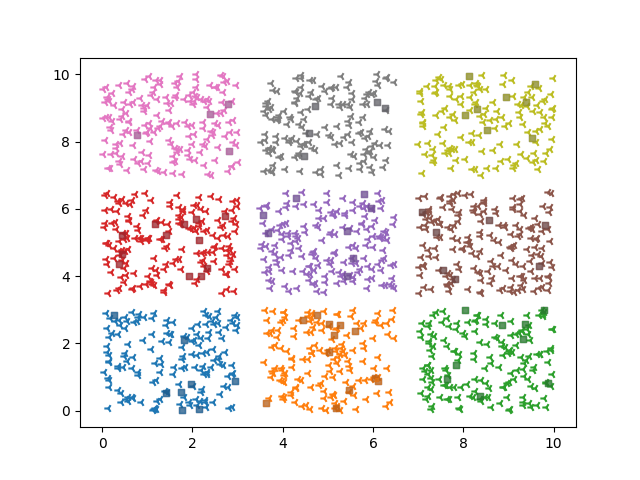
\includegraphics[height=8cm]{Figure_1.png}
        \caption{总样本数为$1800$,样本数为$100$,$k=10$的KNN分类结果。}
    \end{minipage}
 \end{figure}
在实验结果图中,每一个颜色代表一个类别,三叉形点表示训练样本,方形点代表测试样本,方形点的颜色代表了模型的预测结果。最终报告的结果
\begin{minted}[linenos,breaklines,bgcolor=codebg]{c}
total sample number is 1434
total test number is 73
the acc is 1.0
\end{minted}


\subsection*{\Large 附加题一}
{\large\textbf{减少训练样本,增加测试样本(例如n=100,m=500),报告错误率。}}


减少训练样本之后,由于测试样本周围相同类型点变少了,所以这时候位于类区域边缘的点可能会出现误分类的情况。
\begin{figure}[H]
    \centering
    \begin{minipage}[t]{1.0\linewidth}
        \centering
        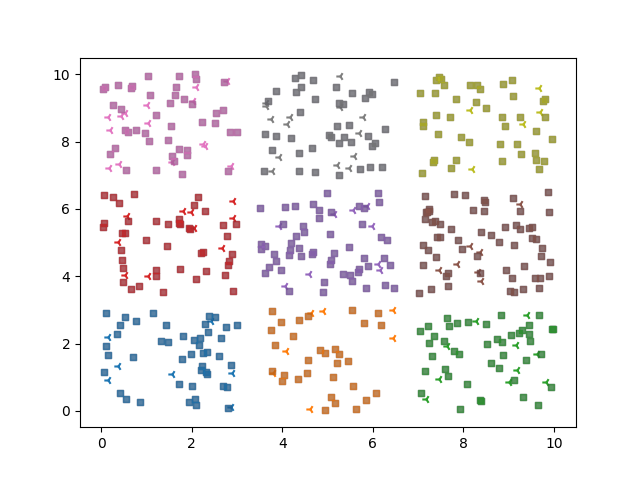
\includegraphics[height=8cm]{add1.png}
        \caption{总样本数为$100$,样本数为$500$,$k=10$的KNN分类结果。}
    \end{minipage}
 \end{figure}
 最终报告的准确率
 \begin{minted}[linenos,breaklines,bgcolor=codebg]{c}
total sample number is 84
total test number is 402
the acc is 0.8830845771144279
\end{minted}

\subsection*{\Large 附加题二}
{\large\textbf{使用不同的度量函数,观测其对分类效果的影响。}}
本次实验中,我们使用了不同的度量函数来计算KNN距离。在总训练样本数$1800$,总测试样本$100$的条件下
三者的预测结果没有区别,这是因为测试样本点的分布比较稀疏。
\begin{figure}[H]
    \centering
    \begin{minipage}[t]{1.0\linewidth}
        \centering
        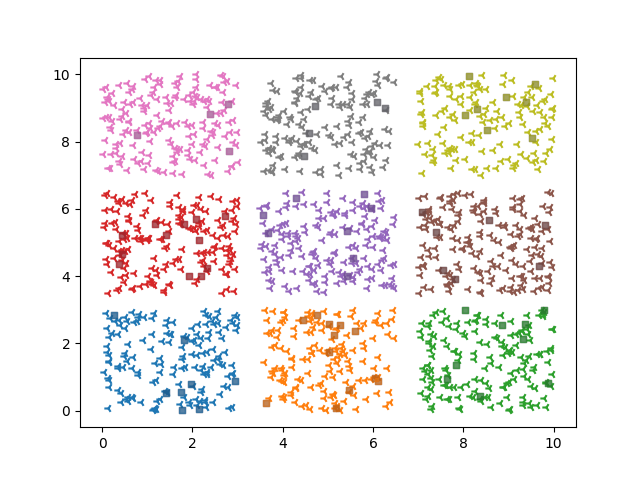
\includegraphics[height=8cm]{eu1.png}
        \caption{训练样本数为$1800$,测试样本数为$100$,$k=10$,度量函数为欧式距离的KNN分类结果。}
    \end{minipage}
 \end{figure}
 \begin{figure}[H]
    \centering
    \begin{minipage}[t]{1.0\linewidth}
        \centering
        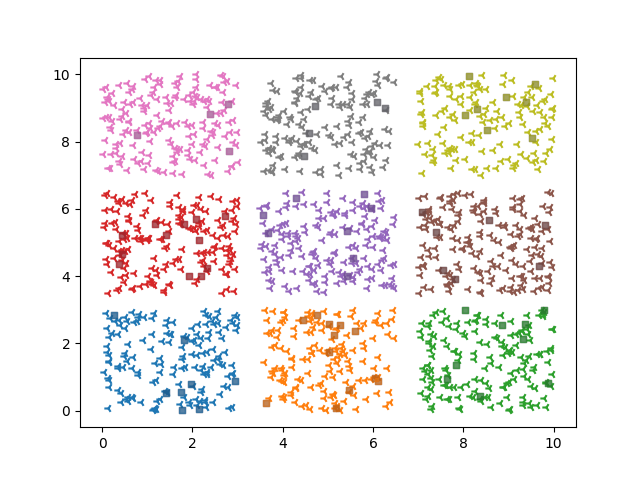
\includegraphics[height=8cm]{man1.png}
        \caption{度量函数为曼哈顿距离的KNN分类结果。}
    \end{minipage}
 \end{figure}
 \begin{figure}[H]
    \centering
    \begin{minipage}[t]{1.0\linewidth}
        \centering
        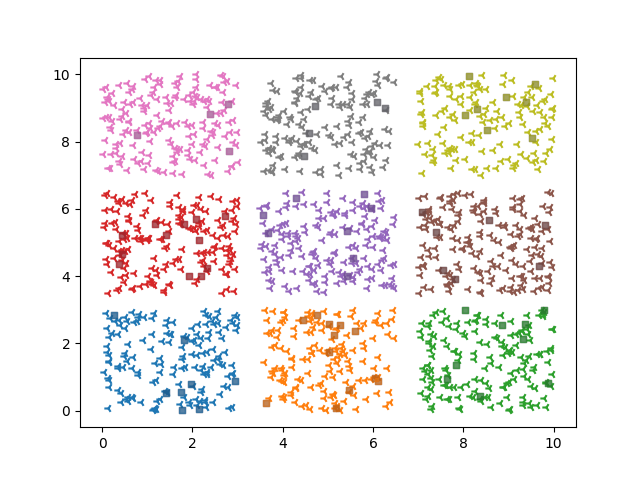
\includegraphics[height=8cm]{inf1.png}
        \caption{度量函数为$p=\infty$的$Minkowski$距离的KNN分类结果。}
    \end{minipage}
 \end{figure}
 三者最终报告的准确率一致
 \begin{minted}[linenos,breaklines,bgcolor=codebg]{c}
total sample number is 1434
total test number is 73
the acc is 1.0
\end{minted}


当我们把训练样本的数量缩小,测试样本数量增大,可以得到不同的结果。
\begin{figure}[H]
    \centering
    \begin{minipage}[t]{1.0\linewidth}
        \centering
        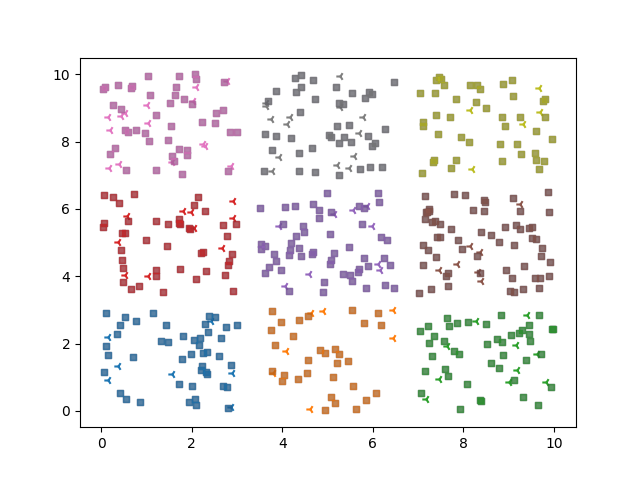
\includegraphics[height=8cm]{eu2.png}
        \caption{训练样本数为$100$,测试样本数为$500$,$k=10$,度量函数为欧式距离的KNN分类结果。}
    \end{minipage}
 \end{figure}
 欧式距离度量时的准确率为
 \begin{minted}[linenos,breaklines,bgcolor=codebg]{c}
total sample number is 84
total test number is 402
the acc is 0.8830845771144279
\end{minted}
 \begin{figure}[H]
    \centering
    \begin{minipage}[t]{1.0\linewidth}
        \centering
        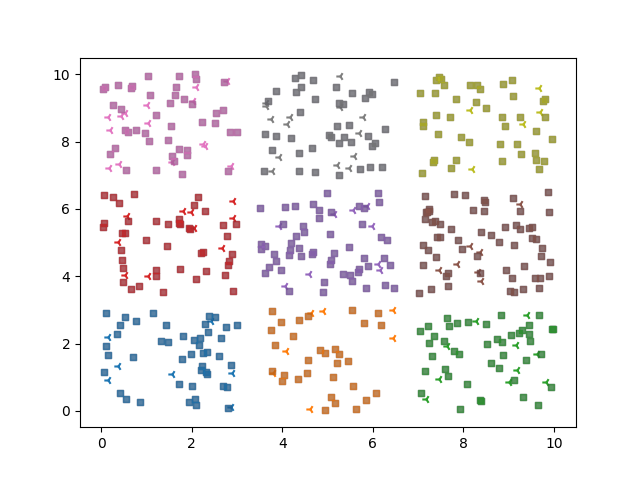
\includegraphics[height=8cm]{man2.png}
        \caption{度量函数为曼哈顿距离的KNN分类结果。}
    \end{minipage}
 \end{figure}
 曼哈顿距离度量时的准确率
 \begin{minted}[linenos,breaklines,bgcolor=codebg]{c}
total sample number is 84
total test number is 402
the acc is 0.9203980099502488
\end{minted}
 \begin{figure}[H]
    \centering
    \begin{minipage}[t]{1.0\linewidth}
        \centering
        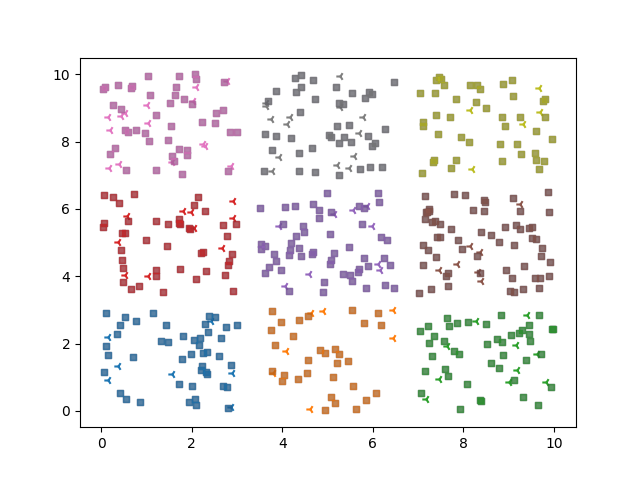
\includegraphics[height=8cm]{inf2.png}
        \caption{度量函数为$p=\infty$的$Minkowski$距离的KNN分类结果。}
    \end{minipage}
 \end{figure}
 $p=\infty$的$Minkowski$距离度量结果
 \begin{minted}[linenos,breaklines,bgcolor=codebg]{c}
total sample number is 84
total test number is 402
the acc is 0.8805970149253731
\end{minted}


实验结论是曼哈顿距离度量的结果更优,对于曼哈顿距离来说,距离某一个特定中心点等距离的其他点构成一个
正方形(欧式距离是一个圆),而我们的样本分布就是一个均匀分布的正方形,很可能与这个分布的形状有关。


\subsection*{\Large 附加题三}
{\large\textbf{思考影响K近邻分类效果的因素有哪些,通过设计特殊的数据分布,实验验证其影响。}}


数据规模首先是一个非常重要的影响因素,这在上面的附加题已经有所论述。
这里我们将原来的均匀分布改为以不同中心点的$\sigma=0.8^2$的正态分布,为了简单起见,我们不再通过原来划分区域的方式来区别不同的类。
首先考虑欧式距离度量的结果,原来的代码修改为:
\begin{minted}[linenos,breaklines,bgcolor=codebg]{python3}
    np.random.seed(25565)
    sample=np.random.rand(100,2)*10
    tag=np.zeros(100)
    test=np.random.rand(500,2)*10
    test_tag=np.zeros(500)
    default_color= ['#1f77b4', '#ff7f0e', '#2ca02c', '#d62728', '#9467bd', '#8c564b', '#e377c2', '#7f7f7f', '#bcbd22', '#17becf']
    
    
    center1=np.array([1.5,1])
    sample1=np.random.randn(600,2)*0.8+center1
    center2=np.array([5,1])
    sample2=np.random.randn(600,2)*0.8+center2
    center3=np.array([8.5,1])
    sample3=np.random.randn(600,2)*0.8+center3
    center4=np.array([1.5,5])
    sample4=np.random.randn(600,2)*0.8+center4
    center5=np.array([5,5])
    sample5=np.random.randn(600,2)*0.8+center5
    center6=np.array([8.5,5])
    sample6=np.random.randn(600,2)*0.8+center6
    center7=np.array([1.5,8.5])
    sample7=np.random.randn(600,2)*0.8+center7
    center8=np.array([5,8.5])
    sample8=np.random.randn(600,2)*0.8+center8
    center9=np.array([8.5,8.5])
    sample9=np.random.randn(600,2)*0.8+center9
    samplen=np.concatenate([sample1[0:100], sample2[0:100], sample3[0:100], sample4[0:100], sample5[0:100], sample6[0:100], sample7[0:100], sample8[0:100], sample9[0:100]])
    testn=np.concatenate([sample1[100:600], sample2[100:600], sample3[100:600], sample4[100:600], sample5[100:600], sample6[100:600], sample7[100:600], sample8[100:600], sample9[100:600]])
    ntag=[]
    ntest_tag=[]
    for k in range(0,9):
        plt.scatter(samplen[k*100:(k+1)*100,0], samplen[k*100:(k+1)*100,1], marker='3', color=default_color[k])
        #plt.scatter(testn[k*500:(k+1)*500,0], testn[k*500:(k+1)*500,1], marker='s', alpha=0.5, s=15, color=default_color[k])
        ntag+=(100*[k+1])
        ntest_tag+=(500*[k+1])
    plt.show()
    total_samplenum=0
    #plt.scatter(sample[:,0],sample[:,1])
    
    def sort_key(item:tuple):
        return item[0]
    
    def knn_predict(point:np.array,n:int)->int:
        dist:list=[]
        for k in range(1,len(samplen)):
            if samplen[k][0]==-1:
                continue
            eu_dis=(samplen[k]-point)@(samplen[k]-point)
            man_dis=np.sum(np.abs(samplen[k]-point))
            inf_dis=np.max(np.abs(samplen[k]-point))
            dist.append((eu_dis,int(ntag[k])))
        dist.sort(key=sort_key)
        vote:list=dist[0:n]
        result=np.zeros(10)
        for j in range(0,len(vote)):
            result[vote[j][1]]+=1
        return result.argmax()
    correct=0
    totalnum=0
    for k in range(0,len(testn)):
        # if testn[k][0]==-1:
        #     continue
        #else:
            ans=knn_predict(testn[k],10)
            plt.scatter(testn[k][0], testn[k][1], marker='s', c=default_color[int(ntest_tag[k]-1)], s=15, alpha=0.5)
            totalnum+=1
            if ans==ntest_tag[k]:
                correct+=1
    plt.show()
    
    #print('total sample number is '+str(total_samplenum))
    print('total test number is '+str(totalnum))
    print('the acc is '+str(correct/totalnum))
    
\end{minted}
生成的训练样本点图像

\begin{figure}[H]
   \centering
   \begin{minipage}[t]{1.0\linewidth}
       \centering
       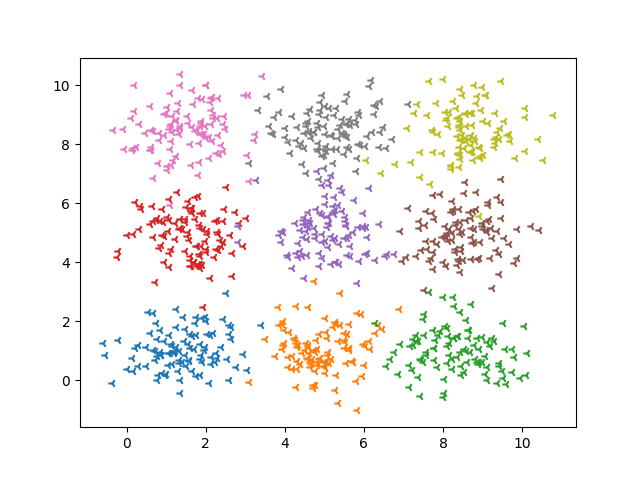
\includegraphics[height=8cm]{normal.png}
       \caption{方差为$\sigma=0.8^2$的不同中心点的正态分布训练样本点。每个类$100$个}
   \end{minipage}
\end{figure}
\begin{figure}[H]
    \centering
    \begin{minipage}[t]{1.0\linewidth}
        \centering
        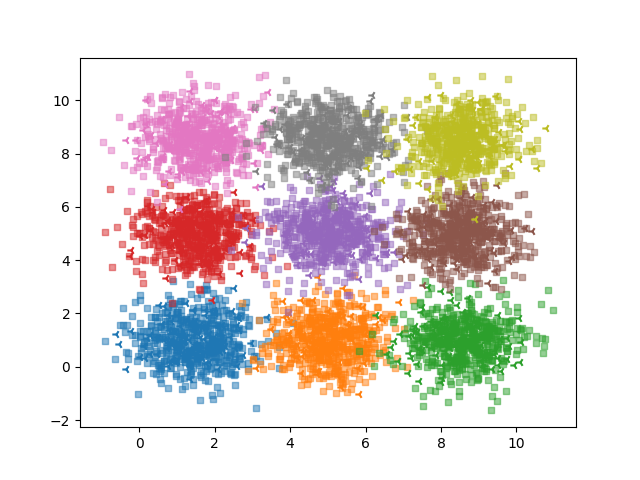
\includegraphics[height=8cm]{normal_with_test.png}
        \caption{同时带有测试样本正确分类和训练样本的图像}
    \end{minipage}
 \end{figure}
使用欧式距离度量的结果为
\begin{minted}[linenos,breaklines,bgcolor=codebg]{python3}
total test number is 4500
the acc is 0.9655555555555555
\end{minted}
预测的各个测试样本点的结果
\begin{figure}[H]
    \centering
    \begin{minipage}[t]{1.0\linewidth}
        \centering
        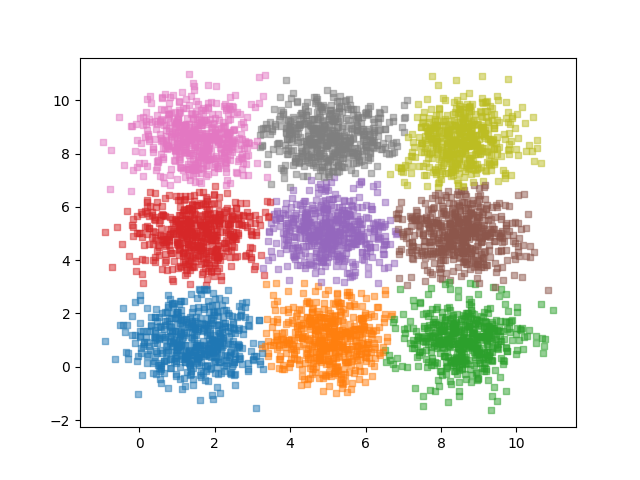
\includegraphics[height=8cm]{normal_pred.png}
        \caption{预测的结果,预测样本每个类$500$个}
    \end{minipage}
 \end{figure}
 使用曼哈顿距离度量的预测结果
 \begin{figure}[H]
    \centering
    \begin{minipage}[t]{1.0\linewidth}
        \centering
        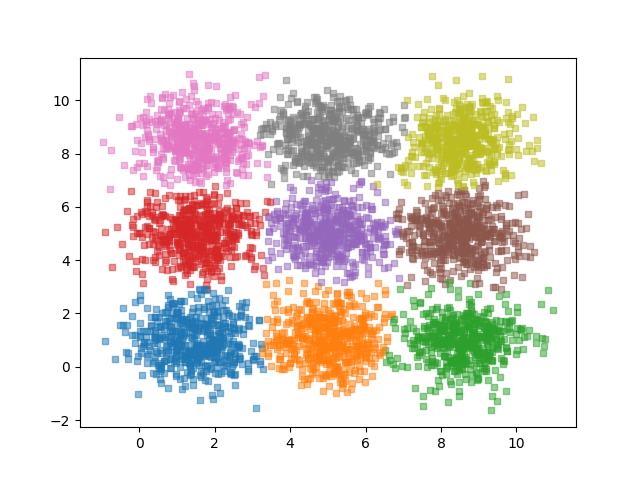
\includegraphics[height=8cm]{normal_man.png}
        \caption{预测的结果,预测样本每个类$500$个}
    \end{minipage}
 \end{figure}
 \begin{minted}[linenos,breaklines,bgcolor=codebg]{python3}
    total test number is 4500
    the acc is 0.9657777777777777
    \end{minted}
使用$p=\infty$的$Minkowski$距离度量结果
\begin{figure}[H]
    \centering
    \begin{minipage}[t]{1.0\linewidth}
        \centering
        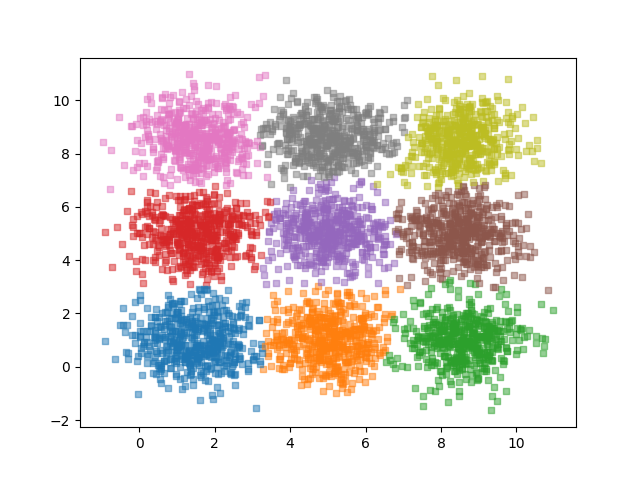
\includegraphics[height=8cm]{normal_inf.png}
        \caption{预测的结果,预测样本每个类$500$个}
    \end{minipage}
 \end{figure}
 \begin{minted}[linenos,breaklines,bgcolor=codebg]{python3}
    total test number is 4500
    the acc is 0.9657777777777777
    \end{minted}


相比于给定范围均匀分布,正态分布的设计更加贴近实际样本的分布情况,因为会出现少量的突变样本,准确率很难到达$1$。我们尝试调大方差的大小为$\sigma=1$得到的结果
\begin{figure}[H]
    \centering
    \begin{minipage}[t]{1.0\linewidth}
        \centering
        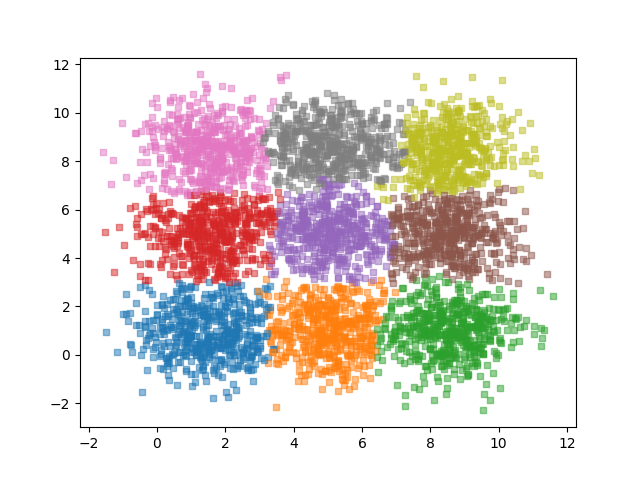
\includegraphics[height=8cm]{sigma1.png}
        \caption{预测的结果,预测样本每个类$500$个}
    \end{minipage}
 \end{figure}
 \begin{figure}[H]
    \centering
    \begin{minipage}[t]{1.0\linewidth}
        \centering
        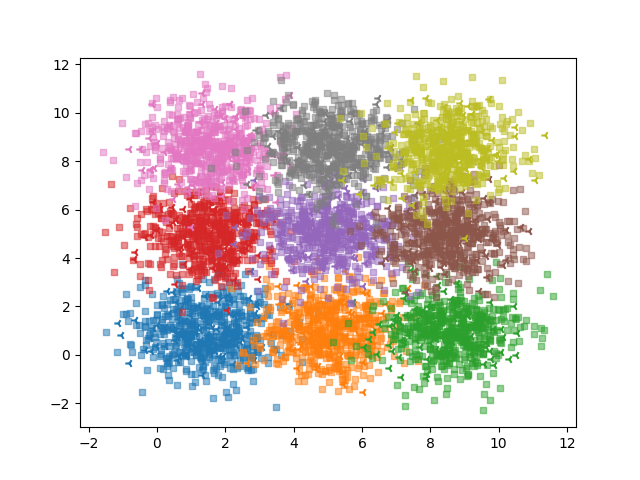
\includegraphics[height=8cm]{sigma1withtest.png}
        \caption{同时带有测试样本正确分类和训练样本的图像(欧式距离),$\sigma=1$}
    \end{minipage}
 \end{figure}
 \begin{minted}[linenos,breaklines,bgcolor=codebg]{python3}
    total test number is 4500
    the acc is 0.908
    \end{minted}
显然随着方差的增大,预测的准确率会下降,这也是符合我们预期的。这时如果我们调高$K$的值为$K=20$
\begin{minted}[linenos,breaklines,bgcolor=codebg]{python3}
    total test number is 4500
    the acc is 0.9106666666666666
    \end{minted}
准确率略有提升,如果我们继续向上调整为$K=25$
\begin{minted}[linenos,breaklines,bgcolor=codebg]{python3}
    total test number is 4500
    the acc is 0.9082222222222223
    \end{minted}


总的来说,调整$K$值一方面可以将更多的样本点纳入考虑范围,使投票结果更具有客观性,但是$K$值并不是越大越好,如果纳入更多的干扰点,
则会导致准确率受到影响。这里其实我们使用正态分布之后,造成不正确的点基本都是突变非常明显的点,这些点周边的小范围内存在大量
与自己不同的其他类型样本,简单的改变范围可能对准确率并没有非常大的影响。不过至少我们可以得出,$KNN$算法最直接的影响因素就是样本
突变程度,这可以用方差来衡量。通过修改$K$值可能可以在小范围内调整这种影响,不过对于方差越大的样本,突变越厉害,也就越难通过调整$K$值
来矫正。
\end{document}



